% !TEX root = main.tex

%%%%%%%%%%%%%%%%%%%%%%%%%%%%%%%%%%%%%%%%%%%%%%%%%%%%%%%%%%%%%%%%%%%%%%%%%%%%%%%%%%%%%%%%%%%%%%%%
\section{理論}
%%%%%%%%%%%%%%%%%%%%%%%%%%%%%%%%%%%%%%%%%%%%%%%%%%%%%%%%%%%%%%%%%%%%%%%%%%%%%%%%%%%%%%%%%%%%%%%%

図1に示す回路で,最初,スイッチSはAの側に倒してあり,
十分長い時間が経過しているものとする.
キャパシタが直流電圧$-V$で充電されている状態で,
時刻$t=0$において,スイッチSをBの側へ切り替えて
直流電圧$V$を印加する.印加される電圧の時間変化は,
図2の階段状の関数で表される.

この場合の回路方程式は,回路に流れる電流を$i(t)$として,$t>0$で
\begin{align}
    L \frac{d i(t)}{d t}+R i(t)+\frac{1}{C} \int i(t) d t=V
\end{align}
となり,これよりキャパシタの電荷$q(t)$に関する微分方程式
\begin{align}
    L \frac{d^2 q(t)}{d t^2}+R \frac{d q(t)}{d t}+\frac{1}{C} q(t)=V
\end{align}
が得られる.

(2)式の2階線形微分方程式は,特性方程式 $L p^2+R p+1 / C=0$ 
の解の判別条件に応じて次の解をもつ.
ただし,$C_1, C_2$は初期条件で決まる定数である.

\begin{enumerate}
    \item $R^2>4L/C$のとき
        \begin{align}
            q(t)=C_1 \exp \{(-\alpha+\beta) t\}+C_2 \exp \{(-\alpha-\beta) t\}+C V
        \end{align}
        \begin{align*}
            ただし \quad \alpha=\frac{R}{2 L}, \quad \beta=\sqrt{\left(\frac{R}{2 L}\right)^2-\frac{1}{L C}}
        \end{align*}

    \item $R^2=4 L / C$ のとき
        \begin{align}
            q(t)=\left(C_1+C_2 t\right) \exp (-\alpha t)+C V
        \end{align}

    \item $R^2<4 L / C$ のとき
        \begin{align}
            q(t)=C_1 \exp (-\alpha t) \sin \left(\beta t+C_2\right)+C V\quad(減㐮振動解)
        \end{align}
        \begin{align*}
            ただし \quad \alpha=\frac{R}{2 L}, \quad \beta=\sqrt{\frac{1}{L C}-\left(\frac{R}{2 L}\right)^2}
        \end{align*}
\end{enumerate}

(5)式は$q(t)=C_1^{\prime} \exp (-\alpha t) \sin \beta t+C_2^{\prime} \exp (-\alpha t) \cos \beta t+C V$
と表すこともできる.

\begin{figure}[H]
    \begin{center}
        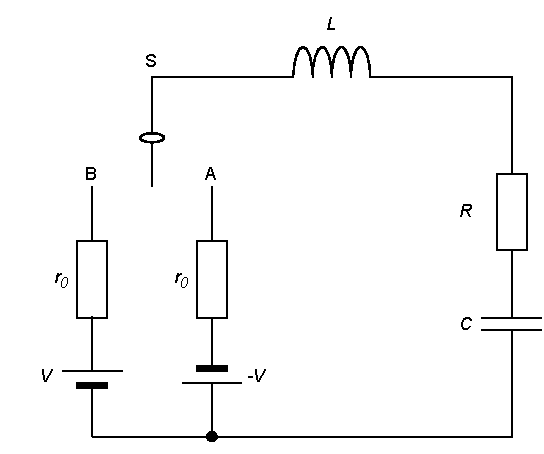
\includegraphics[]{figure1.drawio.pdf}
        \caption{RLC直列回路}
    \end{center}
\end{figure}

\begin{figure}[H]
    \begin{center}
        \begin{tikzpicture}
            \draw[->,>=stealth,semithick] (-pi,0)--(pi,0) node[right]{$t$}; %x軸
            \draw[->,>=stealth,semithick] (0,-2)--(0,2) node[right]{$V(t)$}; %y軸
            \draw[very thick] (-pi,-1) -- (0,-1) node[right]{$-V$} -- (0,1) node[left]{$+V$} -- (pi,1);
        \end{tikzpicture}
        \caption{ステップ関数}
    \end{center}
\end{figure}